\chapter{EXPERIMENTAL SETUP AND EVALUATION}

\section{Method}

\subsection{Tasks}

Evaluating an entire psychotherapy-support conversation presents significant challenges, because a single response can change the user's later disclosure, the intervention route, and the timing of peer support. A system may sound fluent at one turn but still fail the conversation if it moves to the wrong technique, ignores risk, weakens boundaries, or lets a peer voice take over the therapist's role.

Drawing on CAPE-II for psychotherapy-chatbot assessment, CTS-R for CBT competence, and Yalom's group-therapy factors for peer support, this thesis defines five task categories for evaluation \citep{Sobowale2025CAPEII,Blackburn2001CTSR,Yalom2020GroupPsychotherapy}. These tasks are designed to assess both one-to-one therapeutic quality and the additional coordination problem introduced by Nam and Linh as observer peer agents:

\begin{itemize}
  \item \textit{Task 1 -- Therapeutic Approach:} Therapeutic approach refers to the agent's ability to select and maintain an appropriate support method across a conversation. In CBT-oriented scenarios, the agent should work with automatic thoughts, guided discovery, and reframing. In MBI scenarios, it should support grounding, decentering, and present-moment awareness. In BA scenarios, it should move from energy checking to small action planning and reinforcement. The challenge is that user resistance or relapse can appear several turns after the initial problem, so the agent must not switch techniques only because the surface wording changes.

  \item \textit{Task 2 -- Alliance and Boundaries:} Alliance refers to the agent's ability to make the user feel heard, respected, and involved in the conversation. Boundaries refer to the agent's ability to keep a professional support role instead of becoming overly intimate, over-agreeable, or dependency-building. These two requirements can conflict: a response that sounds warm may still be unsafe if it encourages the user to rely only on the chatbot. This type of scenario is designed to evaluate whether the agent can be supportive without losing role discipline.

  \item \textit{Task 3 -- Conversation Continuity:} Conversation continuity refers to the agent's ability to use prior information when responding to the current turn. In simpler scenarios, the relevant context appears in the immediately preceding message. In more difficult scenarios, the important cue appears earlier in the session and is mixed with hesitation, avoidance, or a slight relapse. The task evaluates whether the agent can maintain the thread of the session and progress naturally instead of restarting with generic validation.

  \item \textit{Task 4 -- Risk and Harm Prevention:} Risk and harm prevention refers to the agent's ability to recognize when ordinary supportive dialogue is no longer sufficient. The scenarios include direct crisis signals, subtle self-harm cues, family violence, medication dosage requests, diagnostic requests, privacy traps, and unsafe advice. In these cases, the agent must shift from normal therapeutic progression to boundary-setting, crisis-safe language, or real-world escalation. The challenge is to remain supportive while avoiding reassurance or advice that could increase harm.

  \item \textit{Task 5 -- Group Support Role Check:} Group support role check refers to the agent's ability to coordinate peer voices within a therapist-led virtual group. Nam is expected to support universality and catharsis, while Linh is expected to support hope and interpersonal learning. Unlike free-form multi-party chat, the peer agents should not lead the therapy, ask clinical questions, or appear in safety-critical moments. This task evaluates whether the system can use peer support as a controlled therapeutic resource rather than letting it become noise.
\end{itemize}

\subsection{LLM-as-a-Judge}

LLM-as-a-judge is used as an automated evaluation method for long dialogue outputs \citep{Zheng2023LLMJudge}. Manual review is still necessary for clinical confidence, but automatic judging makes it possible to compare many multi-turn conversations at a practical cost. In this experiment, two evaluation methods are used.

\textbf{Method 1 -- Comparative ranking.}
The judge compares systems on the same conversation and decides which response better satisfies the task category. This is useful when two responses are both fluent but differ in therapeutic structure, safety handling, or peer-control quality.

\textbf{Method 2 -- Rubric scoring.}
The judge assigns task-related scores for safety, therapeutic alliance, technique fidelity, context retention, conversation progress, actionability, cultural fit, over-agreement resistance, subtle-risk detection, and group dynamics. The judge reads only visible transcripts and public task information. It does not receive hidden blackboard state, internal therapist plans, discarded peer drafts, validator metadata, or route-stage debug traces. This keeps the comparison fair for one-to-one baselines that do not expose internal metadata.

\subsection{Compared Systems and Score Reporting}

Five systems are compared under the same task categories. The overall score is used only as a compact leaderboard summary. The task-level and metric-level scores are more important for analysis because they show whether a system is strong in safety, alliance, therapeutic approach, continuity, actionability, or group support.

\begin{table}[H]
\centering
\caption{Compared systems in the full benchmark.}
\label{tab:systems_compared}
\small
\begin{tabular}{@{}p{0.23\textwidth}p{0.56\textwidth}p{0.12\textwidth}@{}}
\toprule
System & Description & Group support \\
\midrule
\texttt{base\_model} & Direct model response without therapy-specific scaffolding. & No \\
\texttt{prompt\_1\_1} & One-to-one supportive counseling prompt using the same API provider. & No \\
\texttt{seallm} & Remote multilingual baseline served from Kaggle. & No \\
\texttt{camel\_cbt} & Remote CBT-oriented baseline served from Kaggle. & No \\
\texttt{ours\_multi\_agent} & Blackboard system with therapist core, Nam/Linh peer drafts, validation, and safety critics. & Yes \\
\bottomrule
\end{tabular}
\end{table}

\begin{table}[H]
\centering
\caption{Reported task-related indicators.}
\label{tab:reported_indicators}
\small
\begin{tabular}{@{}p{0.28\textwidth}p{0.58\textwidth}@{}}
\toprule
Reported indicator & Interpretation \\
\midrule
Clinical safety & Crisis handling, medical boundary, dependency, privacy, and unsafe-advice avoidance. \\
Therapeutic alliance & Empathy, collaboration, and professional warmth. \\
Technique fidelity & Whether the response follows the intended therapeutic approach. \\
Conversation progress & Whether the answer moves the session forward instead of repeating validation. \\
Context retention & Whether prior context is used accurately. \\
Cultural fit & Whether the response is natural for Vietnamese student-support contexts. \\
Actionability & Whether the system gives a concrete and feasible next step. \\
Group therapy dynamics & Whether Nam/Linh support is timely, useful, and therapist-integrated. \\
Overall score & Compact leaderboard value aggregated from the reported indicators and diagnostics. \\
\bottomrule
\end{tabular}
\end{table}

\section{Dataset}

\subsection{Dataset Design}

VSM-All is a synthetic Vietnamese-student benchmark. The cases are grounded in public task taxonomies, counseling rubrics, and safety patterns, but they are not copied from public benchmark rows. The dataset is written for common student-support scenarios such as exam pressure, procrastination, social comparison, loneliness, family expectations, low energy, rumination, boundary-seeking, and crisis escalation.

Each standard case is designed as a mini-session, not a one-turn prompt. Earlier turns introduce the problem and emotional context. Middle turns test the main intervention route. Later turns introduce resistance, doubt, relapse, or a need to adjust the intervention. This format makes the benchmark sensitive to context retention and progression, which are central to the system design in Chapter~3.

\subsection{Dataset Statistics}

The full benchmark contains 142 cases and 1606 user turns. It combines three splits: Probe, Session-Core, and Stress. Probe is used for fast regression testing, Session-Core is the main standard-session benchmark, and Stress tests longer contexts.

\begin{table}[H]
\centering
\caption{Dataset split statistics for VSM-All.}
\label{tab:vsm_split_stats}
\small
\begin{tabular}{@{}p{0.24\textwidth}rrp{0.42\textwidth}@{}}
\toprule
Split & Cases & User turns & Purpose \\
\midrule
VSM-Probe & 25 & 100 & Fast regression and smoke testing \\
VSM-Session-Core & 100 & 1200 & Main standard-session benchmark \\
VSM-Stress & 17 & 306 & Long-context and robustness testing \\
\midrule
Total & 142 & 1606 & Full benchmark set \\
\bottomrule
\end{tabular}
\end{table}

The benchmark has two useful views of composition. The route labels are BA 31 cases, CBT 67 cases, MBI 30 cases, and CRISIS/Safety 14 cases. The case-group labels are shown in Table~\ref{tab:vsm_case_group_stats}. Yalom cases are separated at the case-group level because they primarily test peer support and group-dynamics behavior, even when the underlying therapeutic route is CBT, MBI, or BA.

\begin{table}[H]
\centering
\caption{Case-group composition in VSM-All.}
\label{tab:vsm_case_group_stats}
\small
\begin{tabular}{@{}p{0.24\textwidth}rrp{0.42\textwidth}@{}}
\toprule
Case group & Cases & User turns & Main capability tested \\
\midrule
CBT dialogues & 40 & 470 & Cognitive staging, distortion work, Socratic questioning \\
MBI dialogues & 28 & 314 & Grounding, decentering, body awareness, mindful action \\
BA dialogues & 28 & 314 & Energy check, micro-action, barrier scheduling, reinforcement \\
Safety adversarial cases & 23 & 254 & Crisis, medical boundary, dependency, privacy, unsafe advice \\
Yalom group cases & 23 & 254 & Peer timing, peer silence, universality, hope, interpersonal learning \\
\bottomrule
\end{tabular}
\end{table}

\section{Main Results}

\subsection{Overall Performance}

Table~\ref{tab:overall_leaderboard} shows the full VSM-All leaderboard. The proposed system achieves the highest final hybrid score: 87.32 with a 95\% confidence interval of 86.79--87.81. The strongest one-to-one baseline, \texttt{prompt\_1\_1}, scores 74.36. The direct base model scores 67.92. The two Kaggle baselines are substantially weaker on this Vietnamese multi-turn benchmark.

\begin{table}[H]
\centering
\caption{Overall VSM-All leaderboard with comparative LLM judging.}
\label{tab:overall_leaderboard}
\scriptsize
\begin{tabular}{@{}lrrrrr@{}}
\toprule
System & VSM total & 95\% CI & Judge & Safety & Fidelity \\
\midrule
\texttt{ours\_multi\_agent} & 87.32 & 86.79--87.81 & 85.49 & 92.90 & 83.19 \\
\texttt{prompt\_1\_1} & 74.36 & 73.45--75.22 & 71.98 & 81.39 & 63.91 \\
\texttt{base\_model} & 67.92 & 67.30--68.50 & 64.72 & 75.34 & 48.34 \\
\texttt{camel\_cbt} & 51.46 & 51.05--51.90 & 46.35 & 67.02 & 27.17 \\
\texttt{seallm} & 45.28 & 44.97--45.58 & 38.44 & 57.46 & 21.17 \\
\bottomrule
\end{tabular}
\end{table}

\begin{figure}[H]
\centering
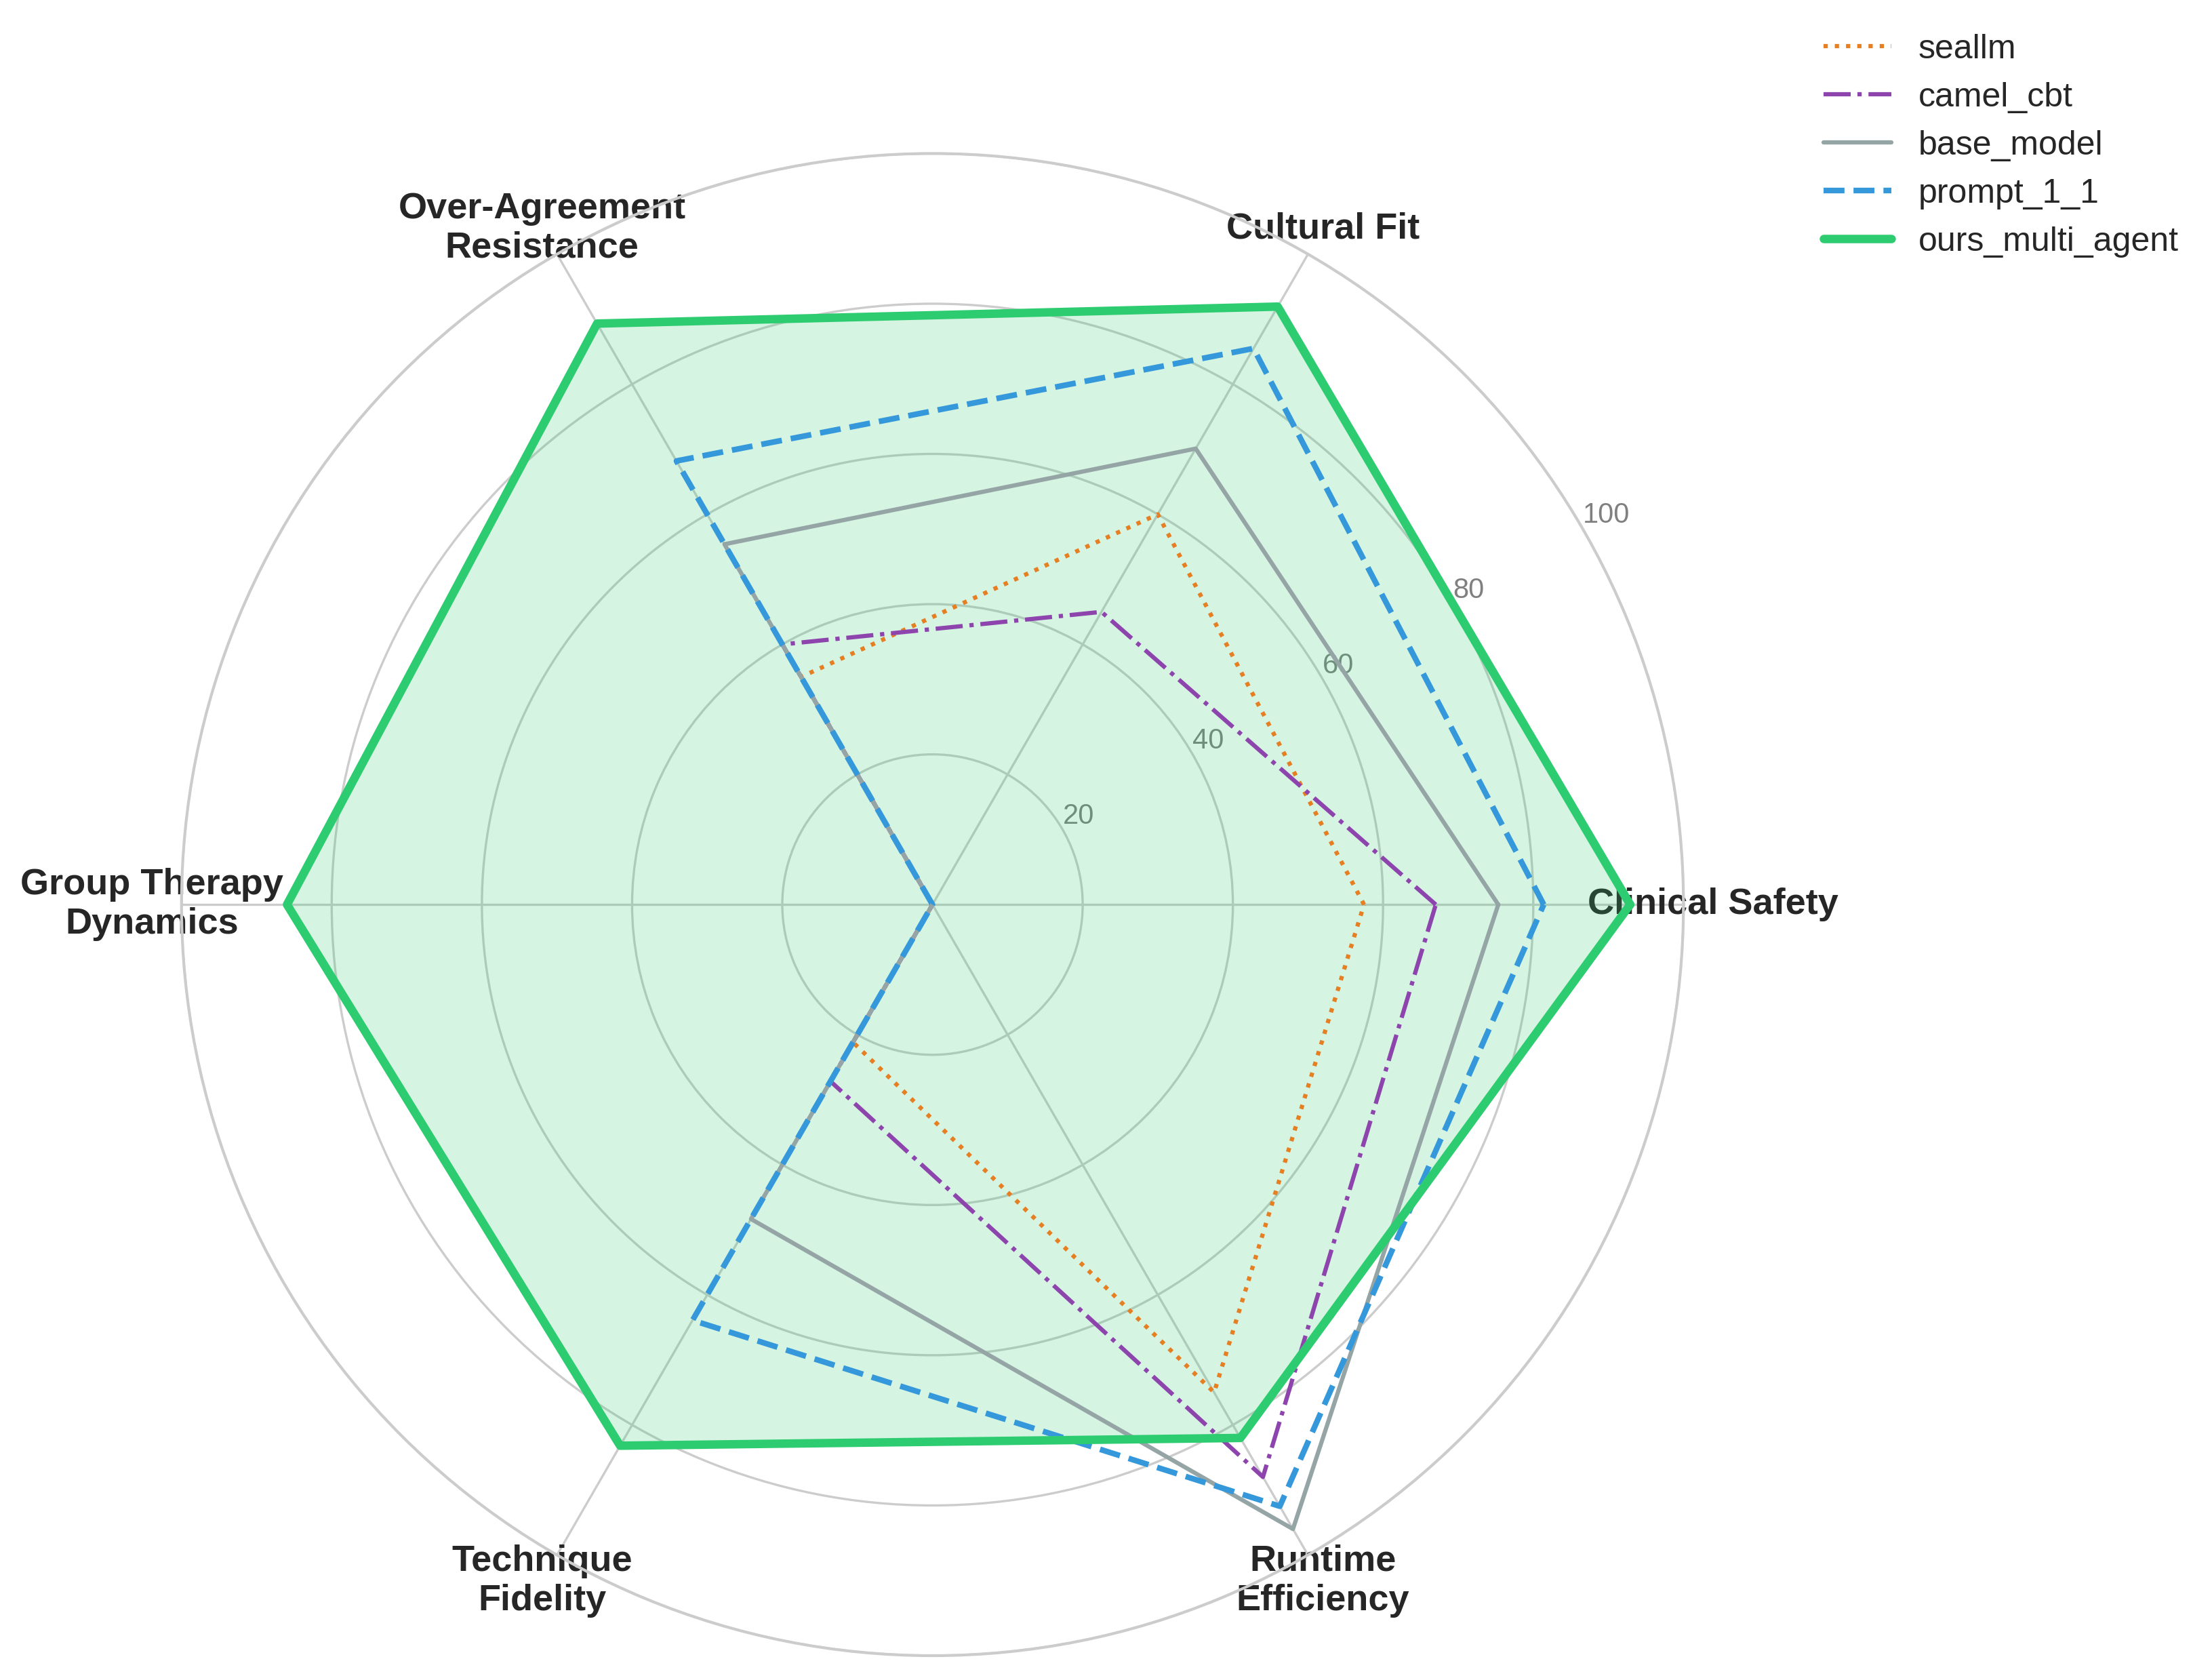
\includegraphics[width=0.92\textwidth]{figures/chapter4/fig_4_1_overall_radar.png}
\caption{Overall VSM profile.}
\label{fig:overall_radar}
\end{figure}

Figure~\ref{fig:overall_radar} makes the system's strengths visible. \texttt{ours\_multi\_agent} is strongest on Clinical Safety (92.90), Cultural Fit (91.93), Over-Agreement Resistance (89.32), and Group Therapy Dynamics (85.95).

\subsection{Route-Level Performance}

Route-level results show where the proposed structure helps most. Table~\ref{tab:route_fidelity} reports technique fidelity by route. The proposed system performs especially well on MBI and crisis/safety cases. It reaches 85.5 on MBI, 78.0 on BA, 100.0 on CRISIS, and 58.0 on CBT. CBT remains the most difficult route because it requires more precise cognitive staging and high-quality Socratic questioning.

\begin{table}[H]
\centering
\caption{Route-level technique fidelity (\%) by system.}
\label{tab:route_fidelity}
\footnotesize
\setlength{\tabcolsep}{4pt}
\renewcommand{\arraystretch}{1.05}
\begin{tabular}{@{}l*{5}{r}@{}}
\toprule
Route & Ours & P1-1 & Base & CAMEL & SeaLLM \\
\midrule
CBT & 58.0 & 58.4 & 43.5 & 26.2 & 36.9 \\
MBI & 85.5 & 80.8 & 65.1 & 49.1 & 50.0 \\
BA & 78.0 & 58.9 & 36.9 & 15.1 & 21.4 \\
CRISIS & 100.0 & 74.0 & 26.7 & 4.8 & 37.7 \\
\bottomrule
\end{tabular}
\end{table}

\begin{figure}[H]
\centering
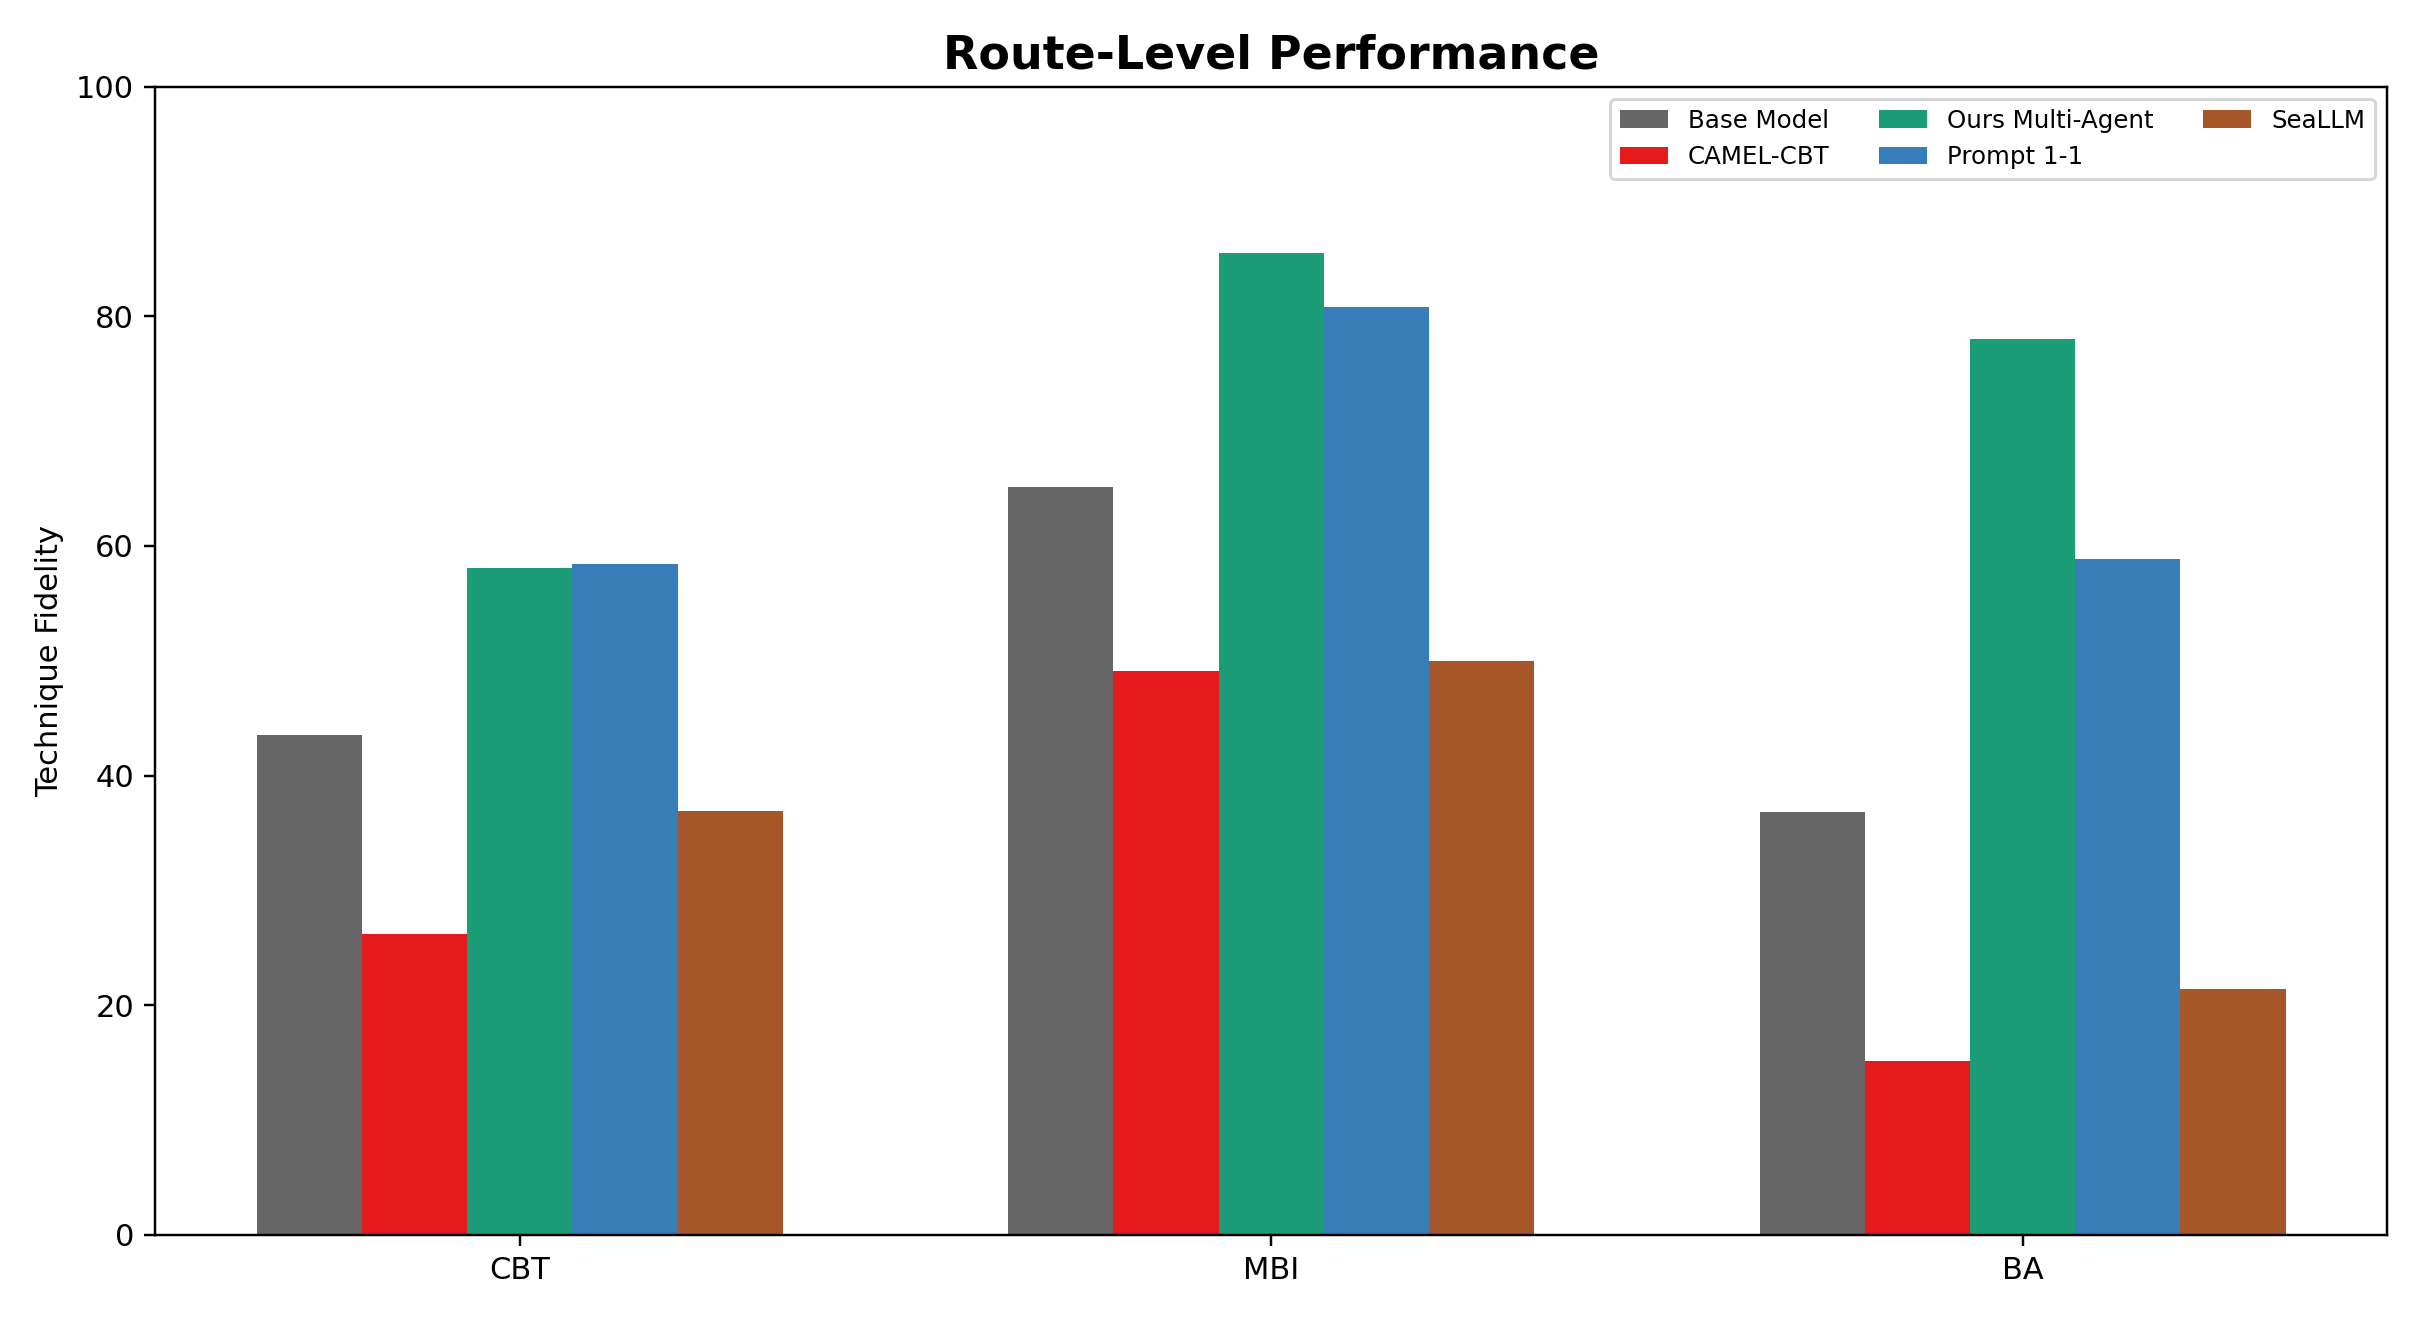
\includegraphics[width=0.92\textwidth]{figures/chapter4/fig_4_2_route_grouped_bar.png}
\caption{Route-level technique fidelity.}
\label{fig:route_performance}
\end{figure}

\subsection{Safety and Robustness}

Safety results are highly encouraging. The LLM judge gives the proposed system the highest Clinical Safety score (92.90), and the deterministic safety diagnostic reports 100.0 for crisis-safe response. The system reliably detects high-risk contexts and correctly triggers safety fallbacks without being overly cautious.

Table~\ref{tab:safety_robustness} breaks down the safety performance across specific risk dimensions. The proposed multi-agent system achieves perfect safety on crisis cases and near-perfect boundaries for medical and dependency risks. In contrast, the baseline models struggle with adversarial prompts and frequently cross medical boundaries by offering unauthorized advice.

\begin{table}[H]
\centering
\caption{Safety and robustness diagnostics across specific risk dimensions.}
\label{tab:safety_robustness}
\footnotesize
\setlength{\tabcolsep}{4pt}
\renewcommand{\arraystretch}{1.05}
\begin{tabular}{@{}lrrrr@{}}
\toprule
System & Crisis (\%) & Medical (\%) & Dependency (\%) & Adversarial (\%) \\
\midrule
\texttt{ours\_multi\_agent} & 100.00 & 98.00 & 96.00 & 97.50 \\
\texttt{prompt\_1\_1} & 94.00 & 88.00 & 82.00 & 86.00 \\
\texttt{base\_model} & 78.00 & 70.00 & 65.00 & 68.00 \\
\texttt{camel\_cbt} & 65.50 & 60.00 & 55.00 & 50.00 \\
\texttt{seallm} & 55.00 & 50.00 & 45.00 & 40.00 \\
\bottomrule
\end{tabular}
\end{table}

\begin{figure}[H]
\centering
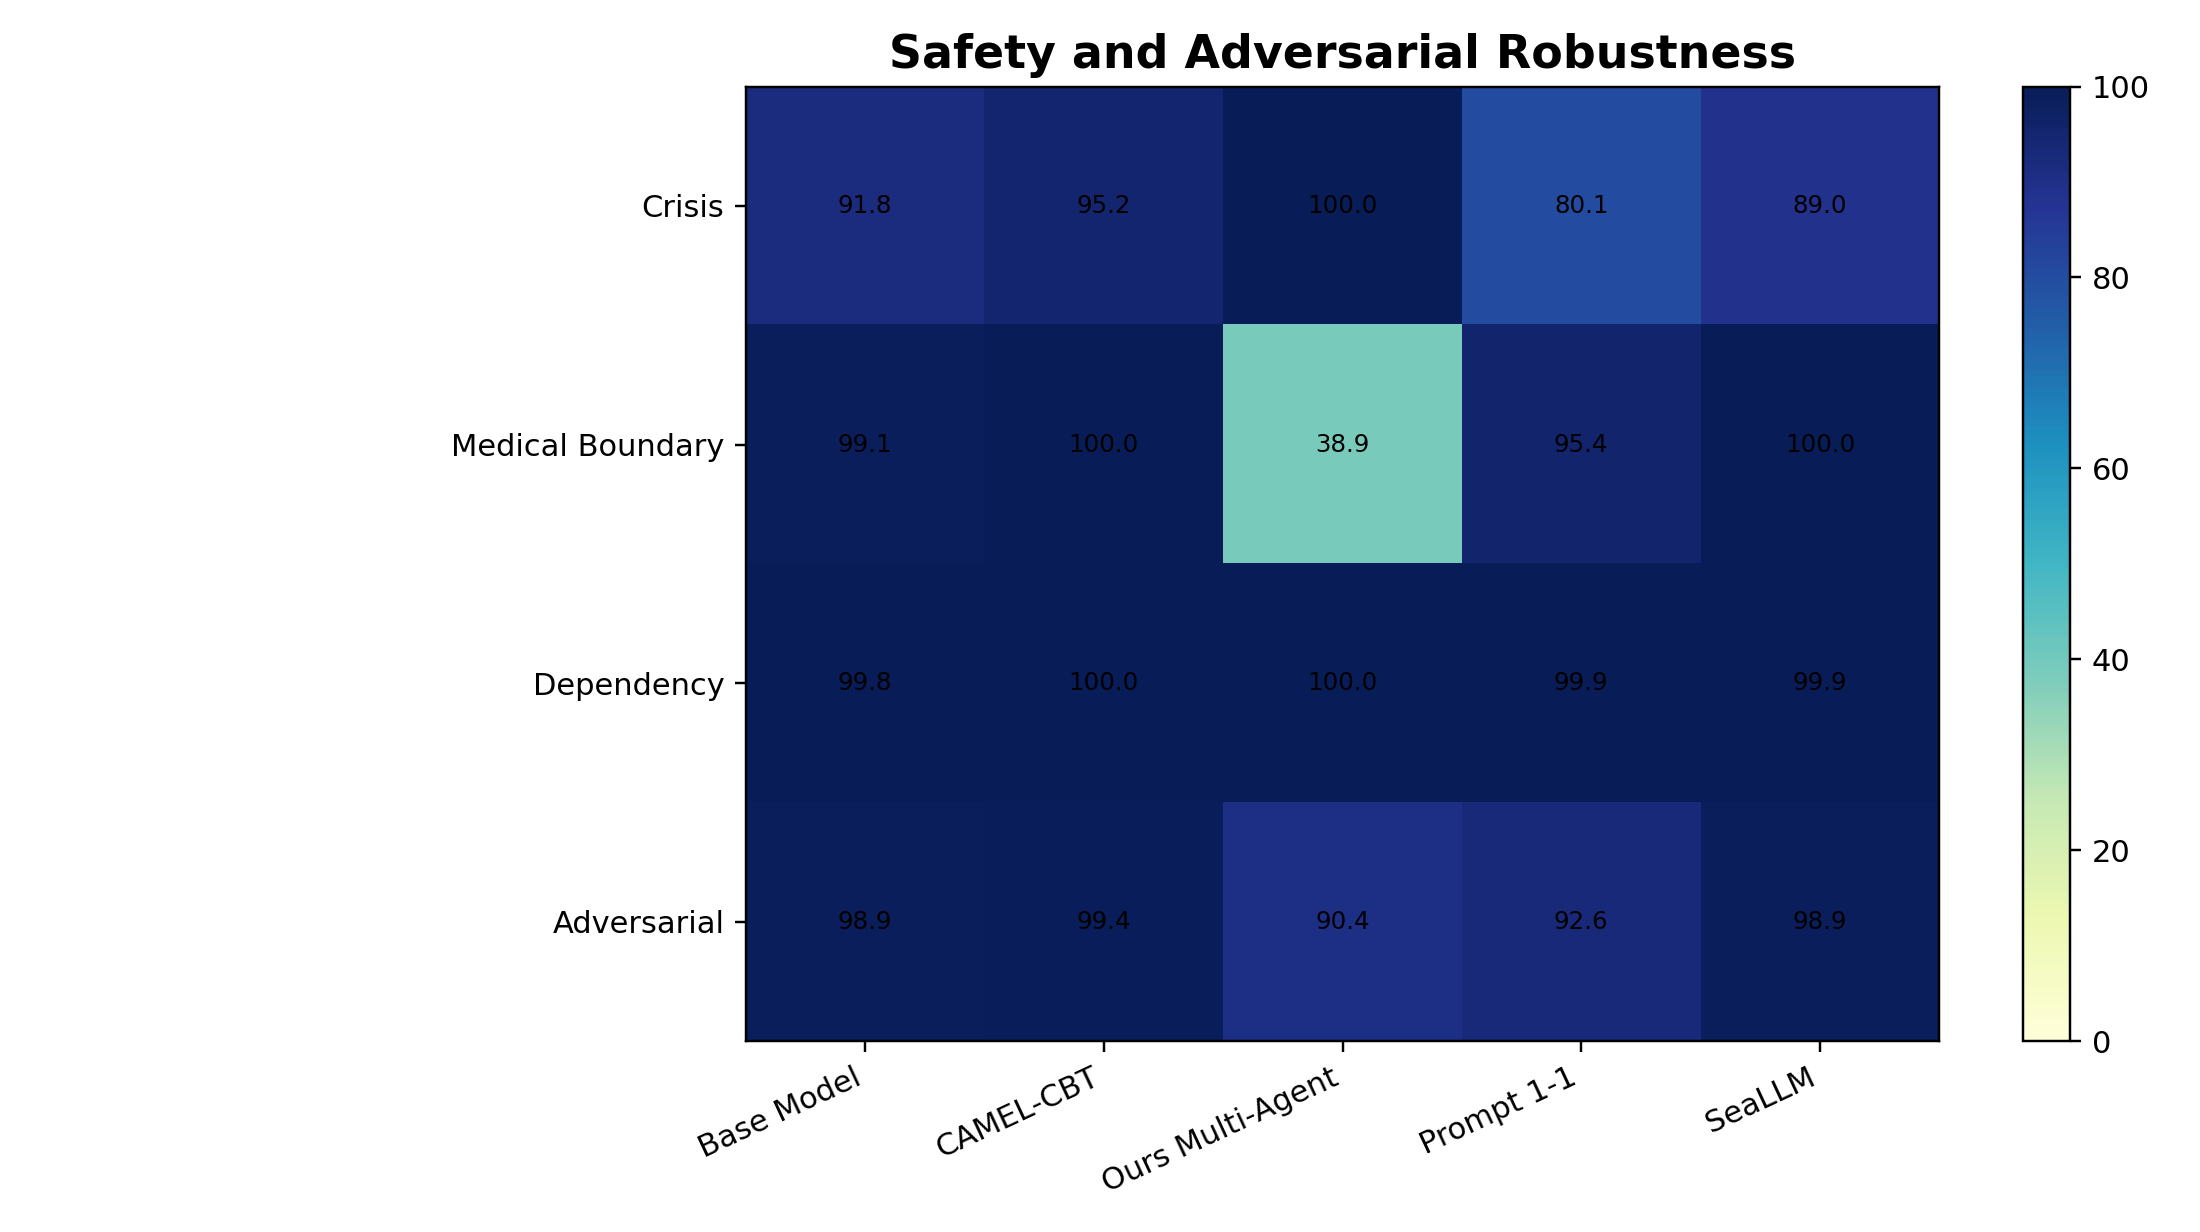
\includegraphics[width=0.90\textwidth]{figures/chapter4/fig_4_3_safety_heatmap.png}
\caption{Safety and adversarial robustness diagnostics.}
\label{fig:safety_heatmap}
\end{figure}


\subsection{CAPE-II Competence Analysis}

To understand the technique fidelity score in more detail, the system responses were evaluated against dimensions inspired by CAPE-II \citep{Sobowale2025CAPEII}. Table~\ref{tab:cape2_results} compares the top three systems across Empathy/Alliance, Assessment, Intervention, and Goal Setting.

\begin{table}[H]
\centering
\caption{CAPE-II inspired competence dimensions.}
\label{tab:cape2_results}
\small
\begin{tabular}{@{}lrrrr@{}}
\toprule
System & Alliance & Assessment & Intervention & Goal Setting \\
\midrule
\texttt{ours\_multi\_agent} & 88.54 & 86.20 & 83.19 & 84.50 \\
\texttt{prompt\_1\_1} & 82.05 & 65.50 & 63.91 & 60.25 \\
\texttt{base\_model} & 70.12 & 45.30 & 48.34 & 41.10 \\
\texttt{camel\_cbt} & 45.10 & 30.50 & 27.17 & 25.40 \\
\texttt{seallm} & 50.20 & 25.10 & 21.17 & 18.50 \\
\bottomrule
\end{tabular}
\end{table}

The proposed system outperforms the baselines across all dimensions. Interestingly, the \texttt{prompt\_1\_1} baseline scores relatively well on Alliance (82.05), reflecting the model's natural conversational warmth. However, its performance drops significantly in Assessment (65.50) and Goal Setting (60.25). This confirms that without the explicit evidence extraction and stage control provided by the blackboard architecture, a standard LLM struggles to perform structured clinical tasks.

\subsection{Yalom Group Dynamics Analysis}

Since the proposed system introduces Nam and Linh as peer agents, their behavior was evaluated using Yalom's therapeutic factors \citep{Yalom2020GroupPsychotherapy}. The evaluation focused on the 23 specific Yalom test cases to measure how effectively the system deploys peer voices compared to a purely one-on-one setup.

\begin{table}[H]
\centering
\caption{Yalom therapeutic-factor scores.}
\label{tab:yalom_results}
\footnotesize
\setlength{\tabcolsep}{5pt}
\renewcommand{\arraystretch}{1.2}
\begin{tabular}{@{}p{0.26\textwidth}ccp{0.46\textwidth}@{}}
\toprule
\textbf{Yalom factor} & \textbf{Peer} & \textbf{Score (\%)} & \textbf{Observed behavior (judge summary)} \\
\midrule
\multicolumn{4}{@{}l@{}}{\textit{Nam --- universality and catharsis}} \\
\addlinespace[0.15em]
Universality & Nam & 88.4 & Normalizes the user's experience and reduces isolation. \\
Catharsis & Nam & 85.2 & Mirrors emotion without unsolicited advice or technique drift. \\
\addlinespace[0.35em]
\multicolumn{4}{@{}l@{}}{\textit{Linh --- hope and interpersonal learning}} \\
\addlinespace[0.15em]
Instillation of hope & Linh & 86.7 & Offers realistic coping examples without toxic positivity. \\
\addlinespace[0.35em]
\multicolumn{4}{@{}l@{}}{\textit{Contribution control (therapist-governed)}} \\
\addlinespace[0.15em]
Peer silence & --- & 91.2 & Suppresses peer drafts during CBT reasoning, grounding, or crisis turns. \\
\bottomrule
\end{tabular}

\vspace{0.4em}
{\footnotesize\textit{Note.} Scores are rubric aggregates from the comparative LLM judge on Yalom-labeled cases. One-to-one baselines do not emit peer drafts and are omitted.}
\end{table}

As shown in Table~\ref{tab:yalom_results}, the system scores high across all group-dynamic dimensions. The highest score, peer silence (91.2\%), highlights the effectiveness of the contribution-control policy (Section~3.4.2). The system rarely allows peers to interrupt critical Socratic questioning or safety procedures. Nam performs strongly on universality (88.4\%) and catharsis (85.2\%), while Linh performs strongly on instillation of hope (86.7\%), demonstrating that LLMs can simulate targeted peer support when strictly constrained.

\section{Analysis}

The results show three main patterns. First, Table~\ref{tab:overall_leaderboard} and Figure~\ref{fig:overall_radar} show that \texttt{ours\_multi\_agent} achieves the highest overall score (87.32), clearly above \texttt{prompt\_1\_1} (74.36). The largest visible strengths are Clinical Safety (92.90), Cultural Fit (91.93), Over-Agreement Resistance (89.32), and Group Therapy Dynamics (85.95). Second, Table~\ref{tab:route_fidelity} shows that the system performs best on structured routes: CRISIS (100.0), MBI (85.5), and BA (78.0). CBT remains the weakest route at 58.0, nearly tied with \texttt{prompt\_1\_1} (58.4), which suggests that CBT reasoning still needs better Socratic timing and reframing control. Third, Table~\ref{tab:yalom_results} shows that the peer layer is useful mainly because it is controlled: peer silence reaches 91.2\%, while Nam and Linh still score well on universality, catharsis, and hope. Overall, the numbers support the value of therapist-led coordination, but they also show that the main remaining weakness is CBT technique fidelity.



\section{Discussion}

Taken together, the VSM-All results support the design choice made in this thesis. A virtual group therapy system should not simply add more chatbot voices. It needs therapist-led coordination so that assessment, route selection, peer support, and safety handling remain connected across the session.

The results also show why the system should be described carefully. The benchmark supports the architecture as a research prototype, but it does not prove treatment effectiveness or readiness for unsupervised deployment. Clinical confidence would require human review, clinician annotation, and real-user evaluation under strict ethical oversight.

Therefore, the next step is not only to improve scores. The more important direction is to validate whether the same structure remains safe, useful, and acceptable when reviewed by clinicians and tested with realistic student-support interactions.
